\chapter{Felhasználói dokumentáció}
\label{ch:user}


\section{Az alkalmazás célja}

Az alkalmazás célja, hogy a felhasználó segítségével membránrendszereket hozzon létre majd szimulálja számításaikat. A membránrendszer egy olyan biológiailag inspirált számítási modell, amely az eukarióta sejtek működését és felépítését követve evolúciós lépéseken keresztül történő információáramlást ír le membránok között. Minden membrán által körbezárt \textit{ún.} régió tartalmaz evolúciós szabályokat, amelyek nem változnak a membránrendszer működése közben. Az információt a rendszerben a régiókban található molekulák, \textit{ún.} objektumok hordozzák. Egy szabály csak akkor tud végbemenni, ha rendelkezésre állnak a szükséges objektumok kellő számban. Ilyen helyzetekben a szabályoknak végre is kell hajtódnia, tehát nem fordulhat elő, hogy minden objektum hozzáférhető, de nem kerül a szabály alkalmazásra. Egy evolúciós lépésben a maximális párhuzamosság elve érvényesül, azaz a szabályok véletszerűen kerülnek kiválasztása, egészen addig, amíg van alkalmazható szabály. Az egyik szimulálható típusú rendszerben megadhatóak olyan speciális szabályok, amelyek alkalmazásának hatására egy membrán feloldódhat, ilyenkor teljes tartalma (benne levő objektumok és régiók) az őt körbevevő régióba kerül. A szabályok között prioritási sorrend is felállítható. A számítás legfontosabb tulajdonsága annak kimenete, amely általában a legkülső régión kívülre (azaz a környezetbe) kijutó objektumok számát jelenti.


\section{Hardver és szoftver követelmények}

A szoftver futtatásához Linux környezetre van szükség, amely támogatja az \verb|ELF| formátumú bináris állományok értelmezését. Ezen felül a futtatási környezetnek rendelkeznie kell \textit{Python interpreterrel}, illetve a \textit{Qt} keretrendszerhez való hozzáférés érdekében \verb|PySide6| modullal. Az utóbbi könnyen megtehető shell környezetben a \verb|pip install PySide6| paranccsal . A program teljes funkcionalitásának kihasználásához a felhasználó számítógépének a bemeneti perifériák közül egérrel és billentyűzettel kell rendelkeznie. A szoftver hardverigénye nem igényel részletesebb specifikációt.


\section{Futtatás}

Mivel a program futtatható állományban kerül a felhasználóhoz, ezért annak az indításhoz elegendő megnyitni a fájlt tartalmazó mappát, majd duplán kattintani a fájlt reprezentáló ikonra. Ugyanez parancssori környezetben is elvégezhető, ilyenkor a terminálban a megfelelő mappába való elnavigálás után a 
\verb|./MembraneSimulator| parancs megadásával futtatható a program.

\section{Grafikus felhasználói felület}

A felhasználó az alkalmazással a grafikus felhasználói felületen keresztül tud kommunikálni, amely a főablakot és az igény szerint megjelenő dialógusablakokat foglalja magába.

\subsection{Főablak}

\begin{figure}[H]
	\centering
	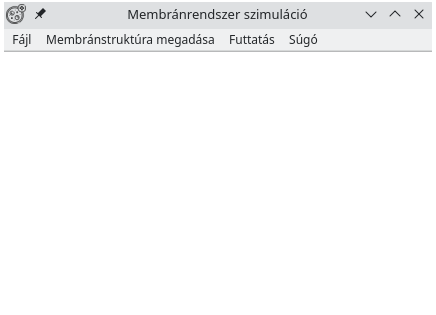
\includegraphics{main_window_empty.png}
	\caption{A főablak az alkalmazás megnyitásakor}
	\label{fig:main_window}
\end{figure}

A főablak az alkalmazás megnyitásakor még tartalmaz egyetlen grafikus elemet sem, viszont a menüsorban található menüpontok segítségével könnyedén változtatni lehet ezen. Ha a felhasználónak nincs korábbi tapasztala a program használatával, akkor érdemes a \textit{Súgó} menüpont kiválasztásával kezdenie, amelyről részletesen szó esik a \ref{help} fejezetben.

\subsection{Dialógusablakok}

A legfontosabb interakció a felhasználó és a szoftver között a dialógisablakokon keresztül történik.  

\subsubsection{Membránstruktúra megadása}\label{create_structure}

Egy membránrendszer megalkotásának kezdeti módja a struktúrájának megadásával kezdődik. Mivel egy membránrendszerben a membránok hierarchikusan helyezkednek el, ezért a teljes rétegződést nagyon jól lehet ábrázolni fa alakban, ahol mindenkinek a szülő csúcsa az őt legszűkebben tartalmazó régió. 

Ezzel egyenértékű az a felírás, amikor egyetlen karakterláncban fejezzük ki ugyanezt, azáltal, hogy egy régiót megfeleltetünk egy nyitó-csukó zárójelpárral. Ilyenkor a két zárójel között elhelyezett objektumok jelentik a régió tartalmát. Azonban nem csak objektumok, de más régiók is helyet kaphatnak, ezzel kifejezve azt, hogy a már említett régió közvetlen gyerekét szeretnénk megadni. 

\begin{figure}[H]
	\centering
	\subcaptionbox{Dialógusablak alapmodell létrehozásához}{
		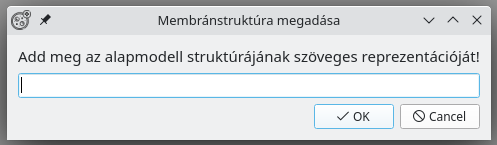
\includegraphics[width=0.4\linewidth]{structure_dialog_base_model.png}}
	\vspace{5pt}
	\subcaptionbox{Dialógusablak szimport-antiport rendszer létrehozásához}{
		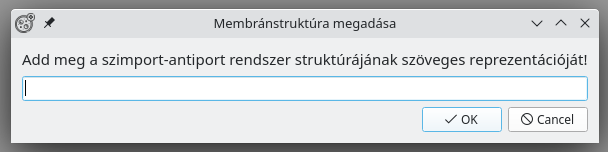
\includegraphics[width=0.45\linewidth]{structure_dialog_symport.png}}
	\caption{Dialógusablakok membránrendszer létrehozásához}
	\label{fig:create_system}
\end{figure}

A \ref{fig:create_system} ábra a különböző típusú membránrendszerek struktúrájának megadásához használt dialógusablakot mutatja. A megadott karakterláncban a régiók kezdetét és végét jelző zárójelpárok, illetve a bennük előforduló objektumok szerepelhetnek.
A helyes formátum feltétele, hogy a zárójelpárok karakterein és az szimport-antiport rendszereknél a kimeneti régió jelzésére használt speciális \textit{\#} karakteren kívül csak az angol ábécé kisbetűi szerepelhetnek a bemenetben, illetve annak meg kell felelnie a helyes zárójelezés szabályainak. Ezt azt jelenti, hogy nem lehetnek átfedések régiók között, azaz olyan karakterláncok, amikor egy külső régió hamarabb kerül lezárásra, mint bármelyik benne lévő régió. Ha ezen feltételeknek megfelel a felhasználó által megadott karakterlánc, akkor a főablak teljes területét lefedő vásznon megjelenik a létrehozott membránrendszer.

Ha a megadott karakterlánc nem a megfelelő formátumú, akkor a felhasználó figyelmeztetésére egy hibaüzenet jelenik meg a képernyőn. 

\begin{figure}
\centering
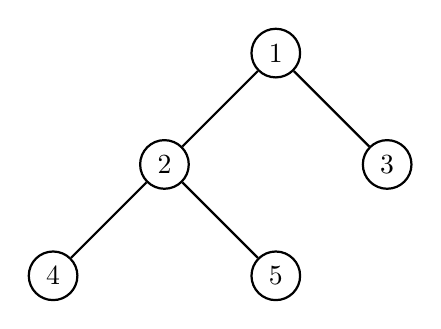
\begin{tikzpicture}[node distance={20mm}, thick, main/.style = {draw, circle}] 
\node[main] (1) {$1$}; 
\node[main] (2) [below left of=1] {$2$}; 
\node[main] (3) [below right of=1] {$3$}; 
\node[main] (4) [below left of=2] {$4$}; 
\node[main] (5) [below right of=2] {$5$}; 
\draw (1) -- (2);
\draw (1) -- (3); 
\draw (2) -- (4); 
\draw (2) -- (5); 
\end{tikzpicture}
\caption{Membránrendszer hierarchikus felépítése\protect\footnotemark}\label{fig:structure_graph}
\end{figure}

\footnotetext{Az ábrán látható struktúra szöveges megfelelője a $[_1 [_2 [_4 ]_4 [_5 ]_5 ]_2 [_3 ]_3 ]_1$ karakterlánc}

\subsubsection{Objektumok módosítása}

Miután a felhasználó megkonstruálta a membránrendszer szerkezetét, utána lehetősége nyílik arra, hogy az egyes régióinak tartalmát szerkessze. Mivel minden egyes régióhoz tartozhatnak objektumok és szabályok is egyaránt, ezért ezek módosítása közös dialógusablakban hajtható végre. A dialógusablak megjelenése a szerkeszteni kívánt régió által lefedett területre történő dupla kattintással kezdeményezhető. 

\begin{figure}[H]
	\centering
	\scalebox{0.8}[0.8]{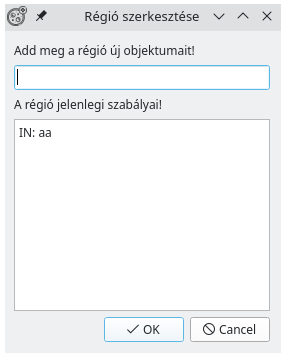
\includegraphics{rule_and_object_edit.png}}
	\caption{Dialógusablak egy régió tartalmának szerkesztéséhez}
	\label{fig:obj_edit}
\end{figure}

A régió objektumai közé tetszőleges számban írható a szóköz, mint elválasztó karakter, amely nem kerül figyelembevételre a régió új objektumainak feldolgozásakor. A megengedett karakterek ezen felül továbbra is az angol ábécé kisbetűi. Ha az adott régió a dialógusablak megnyitásakor már rendelkezik objektumokkal, akkor azok alapértelmezett szövegként fognak szerepelni a szövegdobozban. Tehát ha a régió szerkesztésekor az a felhasználó célja, hogy a kiválasztott régió tartalmát újabb objektumokkal egészítse ki, abban az esetben elegendő a hozzáadni kívánt karakterek begépelése.

\subsubsection{Szabályok módosítása}

A \ref{fig:create_system} segítségével alkotott membránrendszerek még nem fognak szabályokat tartalmazni, ám ezek nélkül nem beszélhetünk még szimulációról.  A szabályok fontos szerepet kapnak az információáramlás vezérlésében, hiszen a hatásukra tudnak objektumok átalakulni, be- és kivándorolni a régiók között. 

\begin{figure}[H]
	\centering
	\subcaptionbox{Régió szabályainak szerkesztése alapmodellben\label{fig:rule_edit_base}}{
		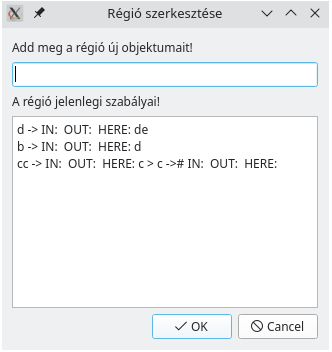
\includegraphics[width=0.45\linewidth]{rule_and_object_base.png}}
	\vspace{5pt}
	\subcaptionbox{Régió szabályainak szerkesztése szimport-antiport rendszerben\label{fig:rule_edit_symport}}{
		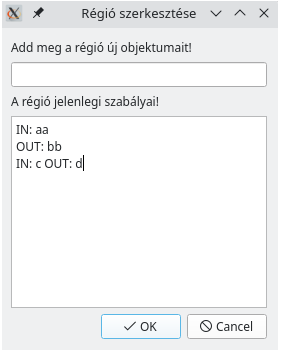
\includegraphics[width=0.38\linewidth]{rule_and_object_symport.png}}
	\caption{Membránrendszerek különböző formátumú szabályokkal}
	\label{fig:rule_edits}
\end{figure}

 A szabályok felépítése függ a membránrendszer típusától. Minden szabály megadása során először fel kell tüntetni, hogy mik azok az objektumok (olyankor ugyanolyan objektumból akár több is egyszerre), amelyek szükségesek a szabály alkalmazásához. 

Szimport-antiport rendszereknél ez a feltétel teljes mértékben elegendő ahhoz, hogy a szabály létrejöjjön, hiszen abban a modellben nincs lehetőség új objektumok létrehozására; a hangsúly inkább az objektumok régiók közötti mozgatására helyeződik. Ahogyan a \ref{fig:rule_edit_symport} alsó szövegdobozában is látható, szimport-antiport rendszerek esetében két különböző típusú szabály hozható létre. Az első a szimport szabály, amelynek két formája van. Az \textit{IN:} kezdetű szabály alkalmazása esetén a kijelölt objektumok a membránt körülvevő tartományból a jelenleg szerkesztés alatt álló tartományba vándorolnak; az \textit{OUT:} kezdetű szabálynál pedig a szerkesztés alatt álló régióból a membránt körülvevő tartományba kerülnek az objektumok. A másik típushoz az ún. \textit{antiport szabályokat}  soroljuk, amelynél egyszerre történik meg az előbbiekkel analóg módon be- és kivándorlás. A bevándorló objektumok előtt az \textit{IN:} prefix szerepel, a kivándorló objektumok pedig az \textit{OUT:} után találhatóak. Ezen két rész a karakterláncon belül felcserélhető, illetve köztük és az objektumok között tetszőleges számú szóköz karakter szerepelhet, amelyek a szabály megalkotásakor nem játszanak szerepet.

Ahogy a \ref{fig:rule_edit_base} ábra is mutatja, az alapmodell esetében a szabályok komplexebb felépítéssel rendelkezhetnek. Első nagy különbség, hogy ebben a modellben objektumok átalakulhatnak, illetve eltűnhetnek vagy megsokszorozódhatnak. Ebben a modellben a szabály alkalmazásához szükséges objektumokat a szabály \textit{bal oldalának} nevezzük. A szabály meghatározása ezen objektumok felírásával kezdődik. A szabály alkalmazásának köszönhetően létrejövő objektumok halmazát a nevezzük a szabály \textit{jobb oldalának}, amelyben az objektumok mozgásának figyelembevételével 3 csoportra bonthatunk:

\begin{compactenum}
	\item Kivándorló objektumok, amelyek a szülő régióba fognak jutni. Ha a legkülső régióban alkalmaztuk a szabályt, akkor az ilyen címkéjű objektumok a környezetbe kerülnek. A szabály megalkotásánál ezen objektumok elé az \textit{OUT:} prefix kerül.
	\item Bevándorló objektumok, amelyek véletlenszerűen valamelyik gyerek régióba fognak kerülni (az alapmodell ennél specifikusabban, címke alapján is megengedi az objektumok mozgását, ezt azonban az alkalmazás nem támogatja). A szöveges formátumban ezen objektumokat az \textit{IN:} szöveg előzi meg.
	\item Régión belül létrejövő objektumok, amelyek a szabályhoz tartozó régióba kerülnek. Ezen objektumok előtt a karakterláncban a \textit{HERE:} kifejezés kell álljon.
\end{compactenum}
A szabály bal és jobb oldalát a \textit{"->"} szimbólumok választják el, amelyek együttesen egy nyilat reprezentálnak, annak kifejezésére, hogy a bal oldalt a jobb oldal objektumai ,,váljták fel''.
Tehát ekkor a \textit{"aa -> IN: bb OUT: cc HERE: dd"} szöveghez tartozó alapmodellbeli szabály két \textit{a} objektumot igényel a végbemeneteléhez (amelyek felemésztődnek a reakció hatására), a régióból kivándorol két \textit{b} objektum, az egyik gyerek régióba bevándorol két \textit{c} objektum, illetve régión belül kialakul két új \textit{d} objektum.

Az alapmodell szabályai kiegészülhetnek többletjelentéssel is. Ebben a modellben ugyanis megengedett lehet egy régió felbomlása, amely egy vagy egyszerre több szabály előidézésére is bekövetkezhet. Ez a szándék jelezhető egy szabály konstruálásakor, ha a bal- és jobb oldalt elválasztó nyilat reprezentáló karakter után közvetlenül egy \textit{\#} karaktert ír a felhasználó. Ilyenkor a régió tartalma és gyerek régiói a szülő régiójába kerülnek.


\subsubsection{Szimulációk számának megadása}

A korábbi dialógusablakok segítségével a felhasználó lehetőséget szerzett arra, hogy a teljes mértékben a saját elképzeléseinek megfelelő membránrendszer hozza létre és konfigurálja fel objektumokkal és szabályokkal. Ezek után már csak a rendszer számításának szimulálása van hátra. A szimulálás végrehajtására két módot biztosít az alkalmazás:

\begin{compactenum}
\item Teljes szimuláció futtatása párhuzamosan tetszőleges számú másolattal 
\item Egy szimulációs lépés az aktuális membránrendszeren
\end{compactenum}

Fontos megjegyezni, hogy a teljes szimuláció futtatásának kiválasztása esetén a képernyőn látható membránrendszer nem kerül szimulálásra, annak érdekében, hogy a szimulálni kívánt állapot megőrződjön, így utána változtatások nélkül kezdeményezhető a funkció megismétlése.

\begin{figure}[H]
	\centering
	\scalebox{1}[1]{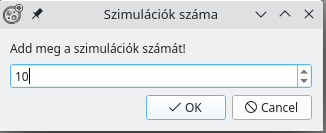
\includegraphics{num_of_simulation.png}}
	\caption{Dialógusablak a szimulációk számának kiválasztásához}
	\label{fig:num_of_sim}
\end{figure}

A szimuláció ismétléseinek számát egy olyan speciális szövegdobozzal lehet beállítani, amely bemenetként csak numerikus értékeket reprezentáló karaktereket fogad el. Alternatívaként a szövegdoboz jobb oldalán található nyilakkal is egyesével állítható az érték, amelynek alsó korlátja \textit{1}, felső korlátja pedig \textit{1000}.
 
\subsubsection{Mentés}
Miután a felhasználó kialakított egy olyan membránrendszert, amelyet szeretne elemezni vagy későbbi használat céljából megőrizni, az alkalmazás lehetőséget biztosít a jelenlegi állapot fájlba történő lementésére.

\begin{figure}[H]
	\centering
	\scalebox{0.5}[0.5]{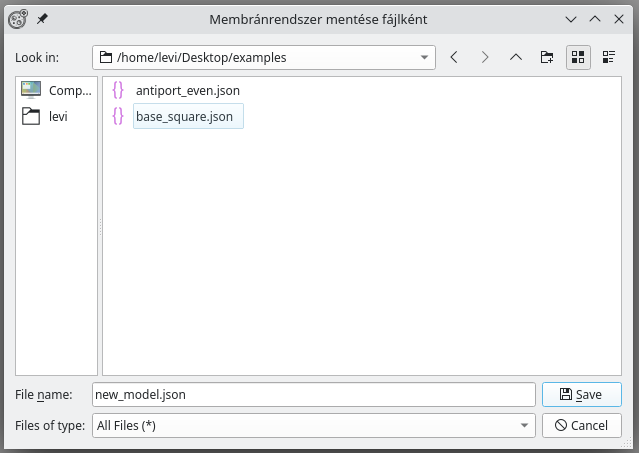
\includegraphics{save_system.png}}
	\caption{Dialógusablak a membránrendszer mentéséhez}
	\label{fig:save_system}
\end{figure}

A mentés folyamata a \textit{Mentés} gombra történő kattintással vagy a \verb| Ctrl+S| billentyűkombináció lenyomásával kezdeményezhető. A funkció kiválasztása után egy dialógusablak jelenik meg, amelyben a mentés helyére kell navigálnia a fájlrendszerben, majd a fájlnév megadása után az \textit{OK} gomb lenyomására létrejön a \textit{JSON} formátumú fájl a megadott útvonallal.

Mivel a \textit{JSON} formátum könnyen értelmezhető és szerkeszthető, ezért egy jártasabb felhasználója a programnak képes egy lementett membránrendszeren módosításokat végezni a megfelelő szerkesztésekkel. 


\begin{figure}[H]
	\centering
	\scalebox{0.4}[0.4]{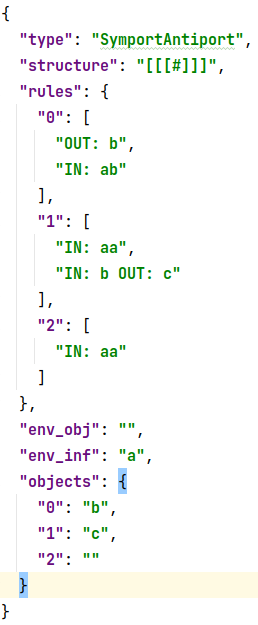
\includegraphics{saved_json.png}}
	\caption{Egy lementett membránrendszerhez tartozó JSON fájl  \protect\footnotemark}
	\label{fig:saved_json}
\end{figure}

\footnotetext{Az ábrán látható konfiguráció a páros számokat generáló szimport-antiport rendszerhez tartozik}

\subsubsection{Betöltés}

Az alkalmazás biztosítja lementett membránrendszerek betöltését, amelynek hatására betöltődik a kiválasztott fájlhoz tartozó állapot a grafikus felületre.
A betöltés nagyon hasonlóan működik a mentéshez, kezdeményezni a \textit{Betöltés} gombra történő kattintással vagy a \verb| Ctrl+O| billentyűkombináció lenyomásával lehetséges, mely után egy dialógusablak segítségével a felhasználó elnavigálhat a megnyitni kívánt fájlt tartalmazó mappához.

\begin{figure}[H]
	\centering
	\scalebox{0.5}[0.5]{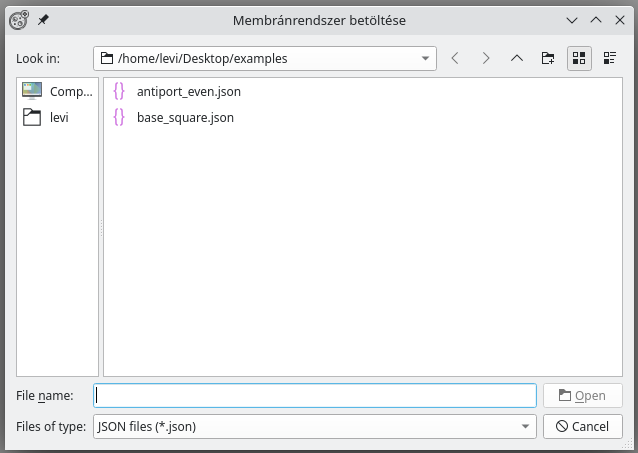
\includegraphics{load_system.png}}
	\caption{Dialógusablak egy membránrendszer betöltéséhez}
	\label{fig:load_system}
\end{figure}

\subsubsection{Eredményablak}

Miután a felhasználó létrehozott egy membránrendszert és szimulálta azt, nincs más hátra mint értesülnie annak eredményéről.  Ezt a funkciót látja el az eredményablak, amely a membránrendszer számításának befejeződése után automatikusan megjelenik és egy listában gyakoriság szerint növekvő sorrendbe rendezve jeleníti meg a különböző számítási eredményeket.

\begin{figure}[H]
	\centering
	\scalebox{0.5}[0.5]{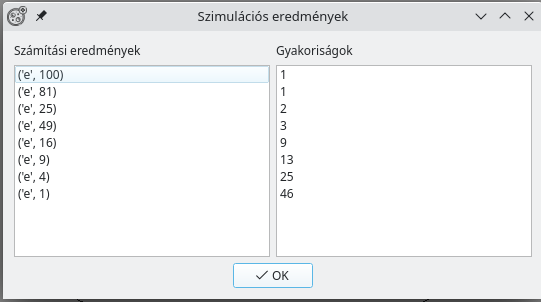
\includegraphics{results.png}}
	\caption{Szimulációs eredményeket kilistázó ablak}
	\label{fig:load_system}
\end{figure}

\section{Használati útmutató}\label{help}

A szoftver használata a membránrendszerek előzetes ismerete nélkül kriptikus tud lenni, ezért a felhasználó útbaigazítására és a szükséges jellemzőkkel kapcsolatos tudnivalók ismertetésére egy súgó funkció is megtalálható a menüsorban.

A \textit{Súgó} gombra való kattintás után jelenik meg az ablak, amelyben a korábbi fejezetekhez hasonló felbontásban találhatóak meg az alkalmazás használatával kapcsolatos információk.

A használati útmutató a \textit{Markdown} formátumnak megfelelő formázásban jelenik meg, amely jól strukturált és könnyen olvasható. A tartalma fejezetekre van bontva, amelyek kitérnek a korábban említett dialógusablakok sajátosságaira, az objektumokkal és szabályokkal kapcsolatos elvárásokra és a szoftver helyes használatának módjára.



A használati útmutató segítségével a felhasználó a membránrendszerekkel kapcsolatos alapvető információkat és a szoftver használatához szükséges tudnivalókat ismerheti meg. A súgó részletes tájékoztatást ad a membránrendszerek létrehozásáról, objektumainak és szabályainak megváltoztatásának módjáról és azok helyes formátumáról, a mentés és betöltés folyamatáról, illetve a számítási eredmény értelmezéséről.

\begin{figure}[H]
	\centering
	\scalebox{0.5}[0.5]{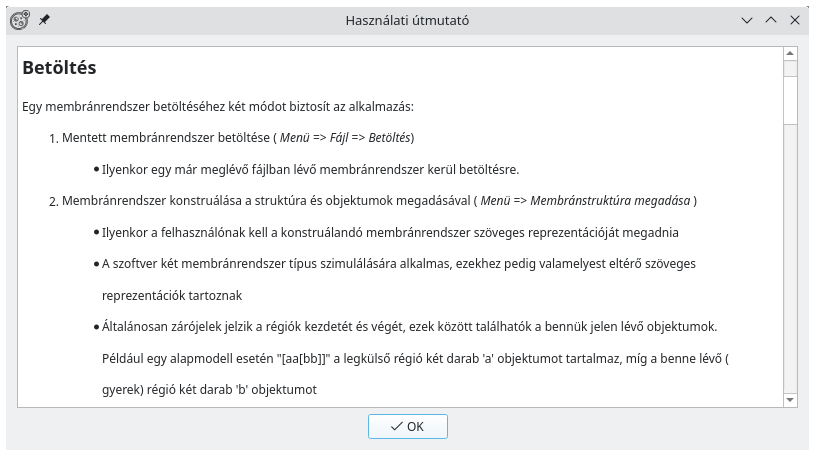
\includegraphics{help_dialog.png}}
	\caption{Használati útmutató ablak}
	\label{fig:help_dialog}
\end{figure}